\chapter{Design}

Once the requirements have been decided, is time to make the design of the system
 that will do all needed to cover them. First we are going to take a look over
 the general arquitecture, the distribution of the domain of the services and
 how delimit their behaviour and communications with each others to after enter
 each one to know how work in each domain and how have been solved all problems
 that this design present.

\section{Responsabilites distribution}

At the moment that we decided split the functionality of the system between
services we found the problem that how decide which is the domain

At the moment that we decided split the functionality of the system between
services, we found the problem that how decide which is the domain of each one.
In the majority of the cases we are begining from a monolithic system that we
want split, in this case is some like this but at first it was thinked to be splited.

In the common app (whatever kind of it) we have three well defined layers, user
interface, logic and storage, something as common MVC\footnote{Model–view–controller
(MVC) is a software architectural pattern for implementing user interfaces on
computers. It divides a given application into three interconnected parts in
order to separate internal representations of information from the ways that
information is presented to and accepted from the user, user interfaces pattern,
introduced by Trygve Reenskaug into Smalltalk-76 at Palo Alto Research Center in the 1970s}
A part of user interface make the necessary to present the info and offer the
way to interact with this to the user while the logic layer do this possible
doing the logic steps to work with data structures saved in some kind of storage.

There are some frameworks as Django wherein all this layer can be developed
toguether, is not strange their popularity, but if we use other as AngularJS
this only help us in the user interface layer, not in the rest, but for other
hands have another advantages.

So, that as it may, this would be the more simple schema to start to work in
our domain, with the difference that we work with service instead of layer in a
single program, but essentially, the concept is the same.

As we can see in the next picture, we will have a user interface, when  will
builded all views and controllers that work with this to buil complete user
interface, a logic section layer, here labeled as APIGmService (as a first
approach) that will do the logic of the system, transform the data,
restructuring and offering the interaction form UI to database.
And at end, the database system, mainly a engine of the database and the drivers
neccesary to work with the.

\begin{center}
\includegraphics[scale=0.3]{img/graphics/initial_microservices_distribution.png}
\end{center}

As we can imagine this work fine, is compact and stable when we are talking about
the same code in the same machine but now we are going to split that in
different services, maybe runing at diferents places and maybe in different
languages, so when we talk about split the domain is about split the logic with
the database access layer.

Next picture show us perfectly what are talking about. This is an example
of migration from monolithic to microservices from Nginx resources.

\begin{center}
\includegraphics[scale=0.4]{img/graphics/refactoring.png}
\end{center}

So, for us, each service will be always mainly the same components,
communication protocol and logic layer. Database layer is always optional,
a service can be do some logic without need a database, imagine a simple service
to do calcs, that consume the data from another service or act as third party
services gateway, a social network, a payment service, whatever.

Coming back again to our problem we have decided to split all the back end in
four services that will cover the domain of the problem, following a Domain
Driven Development principles. Each one will be described with details after,
for now, only a some reasons that why is so. We need a logic part that control
any call to the system, some as gateway that act as dispatcher of request, that
call to the service (maybe not only one) that can help it to resolve the requests
and give back the info. For another and, we need cover all requierements specified,
and to achieve this we  are going to design three services that split all logic
issues, teaching database, students control and analysis microservice. All toguether
compose the backend of the app.

\begin{center}
\includegraphics[scale=0.3]{img/graphics/backend.png}
\end{center}

Further on we will talking about the reason to choose API Gateway as pattern.


Diferents aproximations in the two mainly platforms to work:

\begin{center}
\includegraphics[scale=0.35]{img/graphics/aws_approach.jpg}
\end{center}


\begin{center}
\includegraphics[scale=0.35]{img/graphics/gae_approach.jpg}
\end{center}



This is the complete snap of the system in their final distribution of the
fuctionality between the services.

\begin{center}
\includegraphics[scale=0.22]{img/graphics/final_microservices_distribution.png}
\end{center}

This is the real situation of the develop

\begin{center}
\includegraphics[scale=0.15]{img/graphics/GAE_final_architecture.png}
\end{center}

\subsection{API standar status code cases}

CODIGOS Y POR QUE ELEGIMOS LOS QUE ELEGIMOS



\begin{table}[H]
\centering

\begin{tabular}{@{}lllllll@{}}

Status Code & Meaning\\
\midrule

200 & Ok.The request has succeeded. Information will be returned \\
201 & Created. \\
204 & Ok without body. \\
404 & Not found. \\
422 & Unprocesable entity. \\
500 & Server error. \\

\end{tabular}
\caption{HTTP1.1 Status Code common used}
\label{my-label}
\end{table}

Todo obedecen al estandar y siguen un significado dado por el primer dígito.

\begin{table}[H]
\centering

\begin{tabular}{@{}lllllll@{}}

Class & Meaning\\
\midrule

2xx & Successful\\
3xx & Redirection\\
4xx & Client Error\\
5xx & Server Error\\


\end{tabular}
\caption{HTTP1.1 Status Code common used}
\label{my-label}
\end{table}


\subsection{Pesistence Strategy}

When we are talking aobut persitency that meaning how the data that change
their state in the database is manage. Obviously we are talking of the changes
between created, deleted and the between states.

Is been identified three ways to do this:

1. non persistence
When a item is updated or deleted any information of the last state remain.

2. Half persistence
When a data is logically erased, the data remain in the database but will never
accesible by the user. In this case is isseful if we want develop some mechanism
to redo acctions, in this case only deletion actions.

3. Complete persistence
When not only the elements erased can be restored, all items can be restored in
any point of the hisory of the system. This is the more complex mechanism to persistence
but also the most powerfull and usseful for the users, because as in a simple
text editor allow do an infinite redo over acctions realized.

Afte study all options have been decided use the second approach, and to achieve
this is necessary get some kind of metadata pluged to our objects stored in databases
to control their state in all moment.
To do this has been designed this metadada patter for all objects saved in any
service or database:

\begin{lstlisting}[language=python,frame=none]
  Metadata parameters
  createdBy       INT,
  createdAt       DATETIME,
  modifiedBy      INT,
  modifiedAt      DATETIME,
  deletedBy       INT,
  deletedAt       DATETIME,
  deleted         BOOL,

\end{lstlisting}

With this nosotros coneguios.....


\section{API Gateway microService}

On the other had with docs something similar happens, don't have sense
write a doc defining the behaviour of all sections of api gateway
if this doc already exists in each service. It's redundant and complex
to mantain. Because of this a simple approach is link the docs to
services docs, so the task of write it relegate to them.


\begin{center}
\includegraphics[scale=0.35]{img/graphics/apigateway.png}
\end{center}

\subsubsection {API Definition}






\section{Teaching Data Base microService}

\subsection{Domain and design}

This mService offers the managment of the teaching of the center.
This means that persist in a relational database all relations between
teachers, students, subjects, etc, and all resource availables to
make this posible throuhg an api.\bigskip

This like the rest offers his resource throuhg an api writed in Flask
(follow the same architecture that all).

The engine to save all these relations is MySQL, for many reasons,
mainly because is the best known engine and in which it has some experience
and also because GCP offers as a cloud product Google Cloud SQL Databases.
Until recently only offerts MySQL but now (since March of 2017) they
offer also PostgreSQL.

Access Library design

In the old version it was a little ORM that offers simple methods
to access data transform this in SQL raw sencentes. Now this library
is only a wraper of the SQLAlchemy to keep apart the apirest of the
service to the database access layer.

\begin{center}
\includegraphics[scale=0.35]{img/graphics/tdbms.png}
\end{center}

\subsection{Api definition}
\begin{lstlisting}[language=python,frame=none]

  #%RAML 0.8
  title: Teaching Data Base API
  version: 1.0
  baseUri: ---

  /test:
    description:
    get:
      description:
      responses:
        200:
          description: Ok. Successful requests.

  /test_mysql:
    description:
    get:
      description:
      responses:
        200:
          description: Ok. Successful requests.

  /entities/{kind}:
    description:
    get:
      description:
      responses:
    post:
      description: INSERT a entity in the database, with a special input format:
      responses:

  /entities/{kind}/{entity_id}:
    description:
    get:
      description:
      responses:
        200:
          description:
    put:
      description:
      responses:
        201:
    delete:
      description:
      respones:
        204


  /entities/{kind}/{entity_id}/{nested_kind}/{onk_entity_id}:
  description:

    delete:
      description:
      respones:
        204

  /entities/{kind}/{entity_id}/{related_kind}:
  description:
  get:
    description:
    responses:
      200:
        description:

  /entities/{kind}/{entity_id}/{relared_kind}/{rk_entity_id}/{subrelated_kind}:
  description:
  get:
    description:
    response:
      200:
        description:

  /entities/{kind}/{entity_id}/report:
  description:
  get:
    description:
    response:
      200:
        description:



\end{lstlisting}




\subsubsection{Database logical design}

Based on user histories and the domain of the problem the designe
done based of this entity relation diagram:

The design follow some details that the domain presents, that is related
(at least the more significantly) below:

\begin{center}
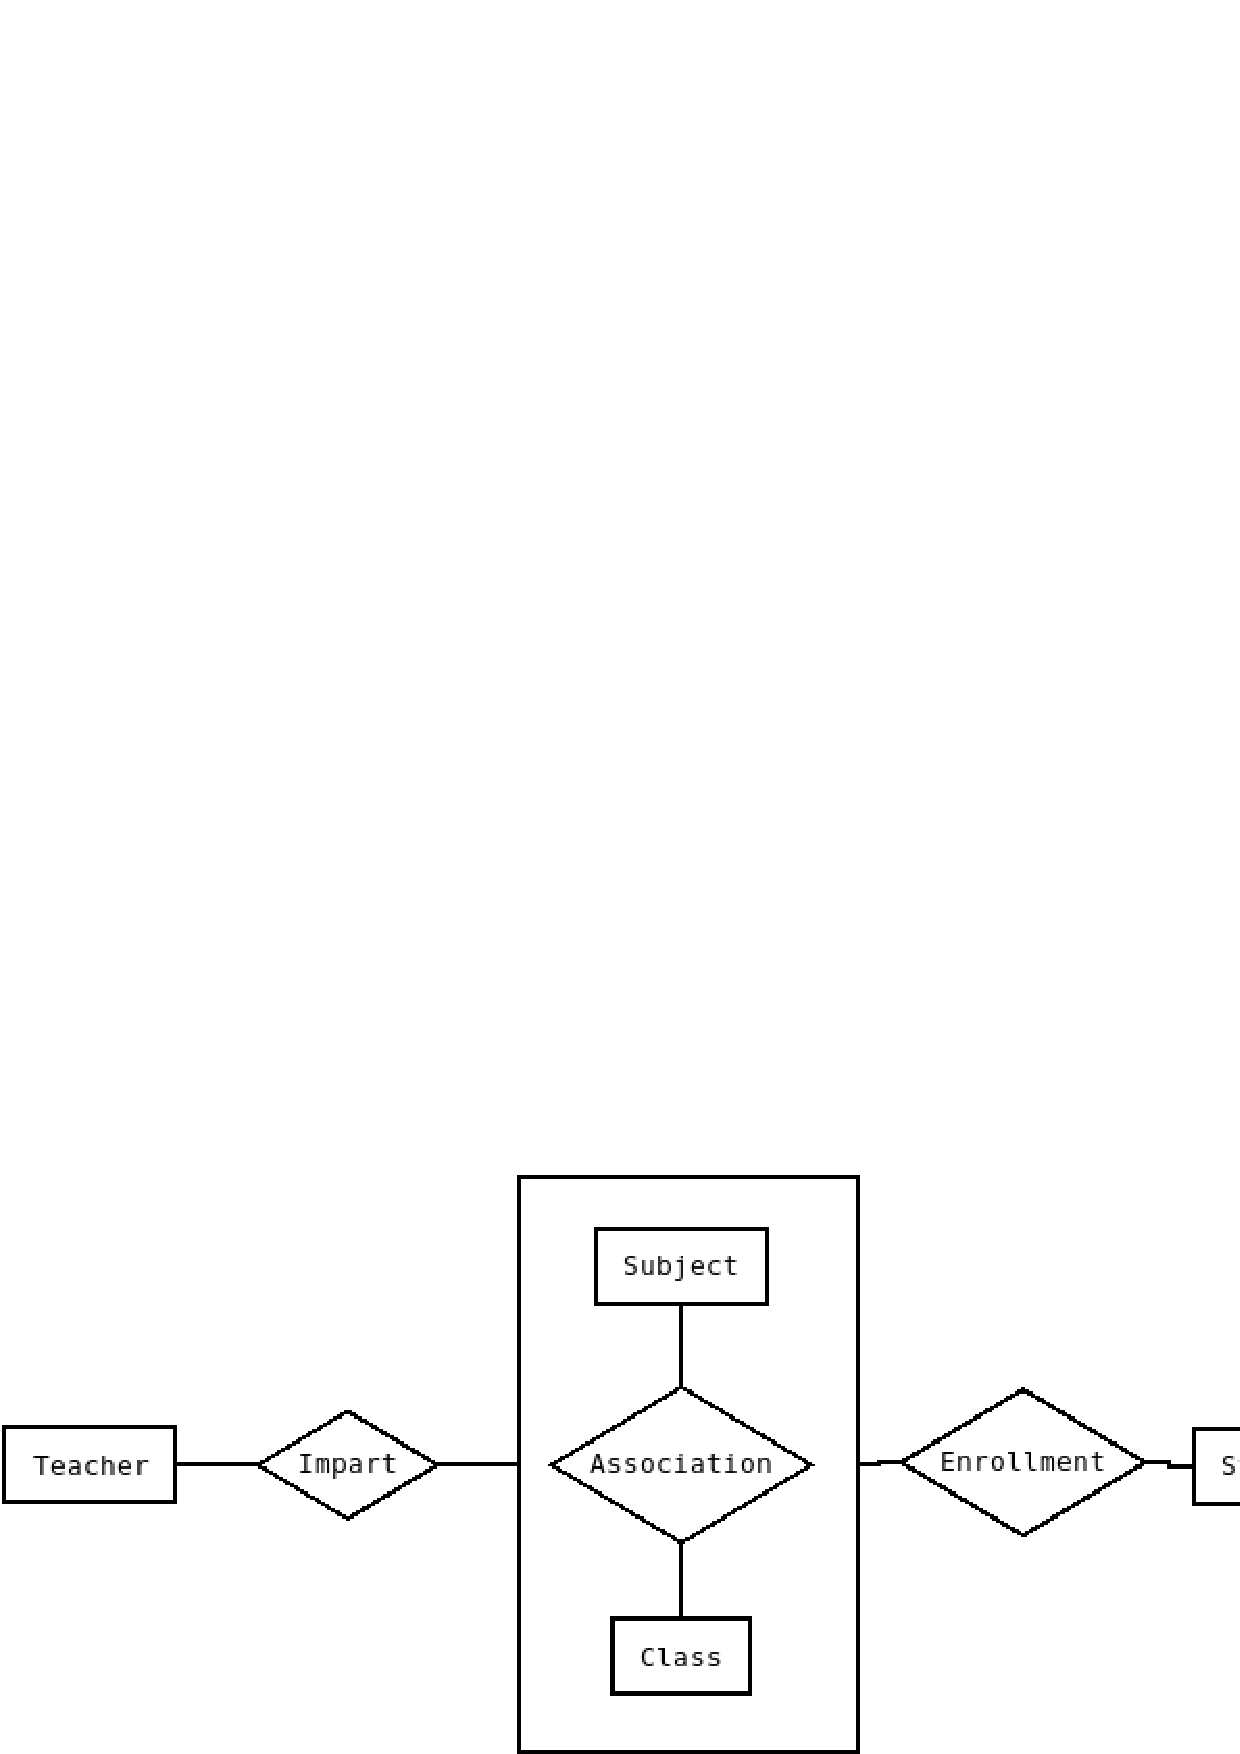
\includegraphics[scale=0.4]{img/diagrams/dbms-ER.png}
\end{center}



\subsubsection{Way to access to raw data}

While at firs of develop the mainly strategie to follow was write
all by cero, finally the point of view has been changed to follow
the use of standard tools and avoid reinvent the wheel.

So, if in the first stages of the project the acces to raw data through
the engine was hand made, using an own simple library that worked
like as simple ORM, the evolution of it and especially the problems
found and the unmaintainability of code have made that now the approach
turned to use a good tool as ORM like \href{http://www.google.es}{SQLAlchemy}.

The changes in the specifications of the api while the develop and
the maintaince of the performance of the queries when is writed hand
made in raw SQL isn't a good idea. Before the develop of this mService
it easy to understand that only in few projects is justified the use
of raw sql sencences and drivers whiout ORM (by easy that it was).


\section{Students Control microService}

\subsection{Domain and design}

\begin{center}
\includegraphics[scale=0.4]{img/graphics/scms.png}
\end{center}

\subsection{Api definition}

skjsñdf
asflkafkdafldañfdsfl


\subsubsection{Attendance Controls Subsection}

This is a simple collection behaviour resource.

This is a RAML0.8 definition file:

\begin{lstlisting}[language=python,frame=none]

  #%RAML 0.8
  title: Attendance Controls API
  version: 1.0
  baseUri: ---
  /ac:
    description: The resource to work with attendance controls database saved-
    get:
      description: Get a list of all attendance controls
      responses:
        200:
          description: Ok. Successful requests. An item will be returned.

    post:
      description:
      responses:
        201:
          description: Created without response. The item was added to database will not
                       returned body.
        422:
          description: Unprocessable Entity. Probably because of the payload
                       sendes has not correct format.

    /{ac_id}:
      uriParameters:
       ac_id:
         displayName: Attendance control ID
         type: integer
      get:
        description: Return an item of the attendance controls collection.
        responses:
          200:
            description: Ok. Successful requests. An item will be returned.
          404:
            description: Not found. The item required does not exists.
      put:
        description: Save a new attendance control in the database.
        responses:
          204: No content. The server has fulfilled the request but does not need to return an entity-body.
          404:
            description: Not found. The item required does not exists.

      delete:
        description:
        responses:
          204: No content. The server has fulfilled the request but does not need to return an entity-body.
          404:
            description: Not found. The item required does not exists.

    /schema:
      uriParameters:
       ac_id:
         displayName: Attendance control ID
         type: integer
      get:
        description:
        responses:
          200:
            description: Ok. Successful requests. An item will be returned.
          404:
            description: Not found. The item required does not exists.

\end{lstlisting}

\subsubsection{Disciplinary Notes Subsection}

This is a simple collection behaviour resource.

This is a RAML0.8 definition file:

\begin{lstlisting}[language=python,frame=none]

  #%RAML 0.8
  title: Attendance Controls API
  version: 1.0
  baseUri: ---
  /ac:
    description: The resource to work with attendance controls database saved-
    get:
      description: Get a list of all attendance controls
      responses:
        200:
          description: Ok. Successful requests. An item will be returned.

    post:
      description:
      responses:
        201:
          description: Created without response. The item was added to database will not
                       returned body.
        422:
          description: Unprocessable Entity. Probably because of the payload
                       sendes has not correct format.

    /{ac_id}:
      uriParameters:
       ac_id:
         displayName: Attendance control ID
         type: integer
      get:
        description: Return an item of the attendance controls collection.
        responses:
          200:
            description: Ok. Successful requests. An item will be returned.
          404:
            description: Not found. The item required does not exists.
      put:
        description: Save a new attendance control in the database.
        responses:
          204: No content. The server has fulfilled the request but does not need to return an entity-body.
          404:
            description: Not found. The item required does not exists.

      delete:
        description:
        responses:
          204: No content. The server has fulfilled the request but does not need to return an entity-body.
          404:
            description: Not found. The item required does not exists.

    /schema:
      uriParameters:
       ac_id:
         displayName: Attendance control ID
         type: integer
      get:
        description:
        responses:
          200:
            description: Ok. Successful requests. An item will be returned.
          404:
            description: Not found. The item required does not exists.

\end{lstlisting}

\subsubsection{Maks Subsection}

This is a simple collection behaviour resource.

This is a RAML0.8 definition file:

\begin{lstlisting}[language=python,frame=none]

  #%RAML 0.8
  title: Attendance Controls API
  version: 1.0
  baseUri: ---
  /ac:
    description: The resource to work with attendance controls database saved-
    get:
      description: Get a list of all attendance controls
      responses:
        200:
          description: Ok. Successful requests. An item will be returned.

    post:
      description:
      responses:
        201:
          description: Created without response. The item was added to database will not
                       returned body.
        422:
          description: Unprocessable Entity. Probably because of the payload
                       sendes has not correct format.

    /{ac_id}:
      uriParameters:
       ac_id:
         displayName: Attendance control ID
         type: integer
      get:
        description: Return an item of the attendance controls collection.
        responses:
          200:
            description: Ok. Successful requests. An item will be returned.
          404:
            description: Not found. The item required does not exists.
      put:
        description: Save a new attendance control in the database.
        responses:
          204: No content. The server has fulfilled the request but does not need to return an entity-body.
          404:
            description: Not found. The item required does not exists.

      delete:
        description:
        responses:
          204: No content. The server has fulfilled the request but does not need to return an entity-body.
          404:
            description: Not found. The item required does not exists.

    /schema:
      uriParameters:
       ac_id:
         displayName: Attendance control ID
         type: integer
      get:
        description:
        responses:
          200:
            description: Ok. Successful requests. An item will be returned.
          404:
            description: Not found. The item required does not exists.

\end{lstlisting}



\section{Analysis microService}

\subsection{Domain and design}
\begin{center}
\includegraphics[scale=0.4]{img/graphics/ams.png}
\end{center}


\section{User Interface microService}

\subsection{Domain and design}
\begin{center}
\includegraphics[scale=0.4]{img/graphics/ui.png}
\end{center}


\section{Auxiliar tools}


\subsection{Provisioner}

A provisioner is simply a tool used to provide a system to insert test data, to avoid to do this hand-made, in our services. Normally this work without knowledge of the internal parts of the backend, only working with their api gateway (or api if we want only fill the database of service), understanding it as black box.
this is only an approach, we can design our provisioner to fill data directly in the databases, which will required stablished a conections with them without the interaction of the services or their connection libraries. This is faster but in some occasions we do not want to do this, because another of their goal is check at the same time the corretly of all parts of apis involved in the data insertion.
So, the execution the this kind of program required that the system has full launched.

This will be the most used tool when we want try some feature that required a lot of data in the system.

How it works?

Easy, only need a simple parameters as entry and based in some rules it will do all calls to the api gateway to insert all data required, besides to save all operations in a register or log file because is necessary to check this in a debug operation.

\begin{center}
\includegraphics[scale=0.4]{img/graphics/provisioner.png}
\end{center}
